
\section{Inner Product Spaces}

\subsection{The Real Dot-Product}

\paragraph{Definition}

For any two vectors \( \vv, vu \) in \( \mathbb{R}^p \), recall that \[
    \vv \cdot \vu = \sum_{i=1}^p v_i u_i
.\]

\paragraph{Positive Definite}
A bilinear map \( T \) is a positive definite if and only if, for all \( \vv \),
\[
    T(\vv, \vv) \geq 0 \quad\text{and}\quad T(\vv, \vv) = 0 \iff \vv = \vec{0}.
\]

\paragraph{Cauchy-Schwarz Inequality}
For any \( \va, \vb \in \mathbb{R}^p \), \[
    - ||\va|| ||\vb|| \leq \va \cdot \vb \leq ||\va|| ||\vb||.
\]

It follows that \[
    -1 \leq  \dfrac{\va \cdot}{||\va|| ||\vb||} \leq 1.
\]

\paragraph{Triangle Inequality}
For any \( \va, \vb \), \[
    ||\va + \vb|| \leq ||\va|| + ||\vb||.
\]

As a vector, the way to think about this is that \( \va + \vb \) is the
hypotenuse between \( \va \) and \( \vb \). It follows directly from
the Cauchy-Schwarz Inequality.

\paragraph{Cosine Angle Between Vectors}
For non-zero \( \va, \vb \), the angle \( \theta \) between \( \va \)
and \( \vb \) is defined with \[
    \cos \theta = \dfrac{\va \cdot \vb}{||\va|| ||\vb||}, \quad \theta \in [0, \pi].
\]

\paragraph{Orthogonality}
Two vectors are orthogonal if and only if \( \va \cdot \vb = 0 \).

\paragraph{Orthonormality}
A set is orthogonal if all elements in it are orthogonal to each other.
A set is orthonormal if it is an orthogonal set and all elements have
unit length.

\paragraph{Orthogonality and Linear Independence}
If a set is orthogonal, then it is linearly independent.

% 
% 
%
\subsection{The Complex Dot Product}

\paragraph{Defining the Complex Dot Product}
For any \( \va, \vb \in \mathbb{C}^p \), \[
    \va \cdot \vb = \sum_{i=1}^p \overline{a_i} b_i = \overline{\va}^{T}B.
\]
That is, take the conjugate of the left term and then apply the real dot
product.

For convenience, define the following shorthand: \[
    \va^* = \overline{\va}^T.
\]

\paragraph{Properties of the Dot-Product}
The complex dot-product has the following properties for all \( \lambda \in \mathbb{C} \)
and \( a, b \in \mathbb{C}^p \):
\begin{itemize}
    \item \( a\cdot (\lambda b + c) = \lambda a\cdot b + \lambda a \cdot c \),
    \item \textbf{Conjugate Symmetry}: \( a\cdot b = \overline{b \cdot a} \)
    \item \textbf{Conjugate Linearity}:
        \( (\lambda a + b) \cdot c  = \overline{\lambda a} \cdot b  + \overline{b} \cdot c\)
    \item \( ||a|| \) is a positive definite.
\end{itemize}

Note that for the real-case conjugate symmetry and conjugate linearity
are just symmetry and linearity. The mix of linearity in the second argument
and conjugate linear in the first argument is called \underline{sesquilinearity}.

Further, the triangle and Cauchy-Schwarz inequalities hold for the complex
case too.

These properties exist to satisfy that the dot-product is an inner-product.

%
%
%
\subsection{Inner Product Space}
Let \( V \) be a vector space over \( \mathbb{F} \)
(typically let \( \mathbb{F} = \mathbb{C} \) unless stated otherwise).

Then an inner product is a mapping \( \innerprod{}{} \) from \( V \times V \)
to \( \mathbb{F} \) that satisfies the following properties for all \( \lambda \in \mathbb{F} \)
\begin{enumerate}
    \item \( \innerprod{u}{v + w} = \innerprod{u}{v} + \innerprod{u}{w} \),
    \item \( \innerprod{u}{\lambda v} = \lambda \innerprod{u}{v}\),
    \item \( \innerprod{v}{u} = \overline{\innerprod{u}{v}} \),
    \item \( \innerprod{v}{v} \) is a real, positive definite.
\end{enumerate}

Observe that this is just a sesquilinear, conjugate symmetric, real positive definite.
The dot-products are examples of inner products.

\paragraph{Standard Inner Product for Continuous Functions}
The inner product over \( \mathcal{C}[a, b] \) is defined as \[
    \innerprod{f}{g} = \int_a^b f(x) g(x) dx.
\]

%
%
%
\subsection{Orthogonality}
For an inner-space \( V \), two non-zero vectors \( u, v \in V \) are orthogonal if
and only if \( \innerprod{u}{v} = 0 \).
Notate this as \( u \perp v \).
The usual definitions for othogonal and orthonormal sets holds.

\paragraph{Projections}
For \( \vu, \vv \in V \), we define the projection of \( \vu \) onto \( \vv \)
as \[
    \proj_{\vv}(v) = \dfrac{
        \innerprod{\vv}{\vu}
    }{
        \innerprod{v}{v}
    } \vv
\]
Note that projection is linear.

Also note that \( \vu - \alpha \vv \) if and only if \[
    \vu - \alpha \vv = \vu - \proj_\vv(\vu)
\]

\paragraph{Orthogonal Sets as Spans}
Suppose that \( V = \set{v_1, \dots, v_k} \) is an orthogonal set.
Then it is also a linearly independent set and so for any \( \vv \in V \)
we can write \[
    \vv = \sum_{i=1}^k \alpha_i v_i. 
\] for unique \( \alpha_i \).

For our orthogonal sets, \[
    \alpha_i = \dfrac{\innerprod{\vv_i}{v}}{||v_i||^2}.
\]
If the set is orthonormal, then we can simplify this to \[
    \alpha_i = \innerprod{\vv_i}{v}.
\]

Alternatively, for the orthogonal case, \[
    \vv = \sum_{i = 1}^{k} \proj_{\vv_i}(\vv).
\]

\subsection{Gram-Schmidt Process}

\paragraph{Existence of Orthonormal Bases}
Any finite dimensional, inner-product space \( V \) has an orthonormal basis.
We can construct this basis using the Gram-Schmidt process.

\paragraph{The Process}
Suppose that \( S = \set{v_1, \dots v_k} \) is a basis for some \( V \)
over \( \mathbb{F} \).
Then, we can construct an orthonormal basis \( S' = \set{w_1, \dots, w_k} \)
that independently spans \( V \) with the following formula: \[
    w_{i} = v_{i} - \sum_{j = 1}^{i - 1} \proj_{w_j}(v_i).
\]

\paragraph{Expansion over \( \mathbb{R}^3 \)}
Let \( \set{v_1, v_2, v_3} \) be an orthogonal set spanning \( \mathbb{R}^3 \).
Then the corresponding orthonormal set is \( \set{w_1, w_2, w_3} \) where
\begin{align*}
    \vw_1     &= \vv_1, \\
    \vw_2     &= \vv_2 - \proj_{\vw_1}(\vv_2), \\
    \vw_3     &= \vv_3 - \proj_{\vw_1}(\vv_3) - \proj_{\vw_2}(\vv_3).
\end{align*}

%
%
%
\subsection{Orthogonal Complement}


\paragraph{Orthogonal Complement}
Let \( X \) be a subspace of some vector space \( V \).
Then, the orthogonal complement \( X^\perp \) is the set where
every element of \( X^\perp \) is orthogonal to \( X \).
That is \[
    X^\perp = {\vy : \vy \cdot \vx = 0 \quad \forall \vx \in X}.
\]

\paragraph{Orthogonal Complements as Direct Sum}
For any subspace \( V \), \[
    V = X \oplus X^\perp, \quad\text{and}\quad {\left(X^\perp\right)}^\perp = X.
\]

Then, for any \( \vv \in V \), we can write the following for unique
\( \vx, \vy \): \[
    \vv = \vx + \vy, \quad \vx \in X, \vy \in X^\perp.
\]

Annotate this as \( \vx = \proj_X(\vv), \vy = \proj_{X^\perp}(\vv) \).

\paragraph{Projection on Subspace}
From the previous result, for any subspace \( W \) with orthogonal basis,
we calculate the projection
onto that as follows: \[
    \proj_{W}(\vv) = \sum_{i = 1}^{k} \proj_{\vw_i}(\vv).    
\]
This follows directly from linearity of projection and the result of orthogonal
sets as spans.


\paragraph{Properties of the Projection Function}
Suppose that \( W \) is a subspace of \( V \) with \( \vv\in V, \vw\in W \).
Then,
\begin{itemize}
    \item \( \vv - \proj_{W}(\vv) \) is in \( W^\perp \),
    \item \( \proj_W(\vw) = \vw \).
    \item The projection mapping is idempotent. That is \( \proj_W \circ \proj_W = \proj_W \).
    \item Projection does not extend lengths. That is, \( ||\proj_W(\vv)|| \leq ||\vv|| \).
    \item \( \proj_W + \proj_{W^\perp} \) is an identity mapping.
\end{itemize}

\paragraph{Projection Minimises}
Recall that projection does not extend lengths.
In-fact we extend this to note that projection will actually minimise the length of
the difference between the original vector and the projection.
That is, \( \vv - \proj_W(\vv) \) is the shortest distance between \( \vv \)
and \( W \).
Consequently, \[
    ||\vv - \vw|| \geq  ||\vv - \proj_W(\vv)||
\]

\begin{center}
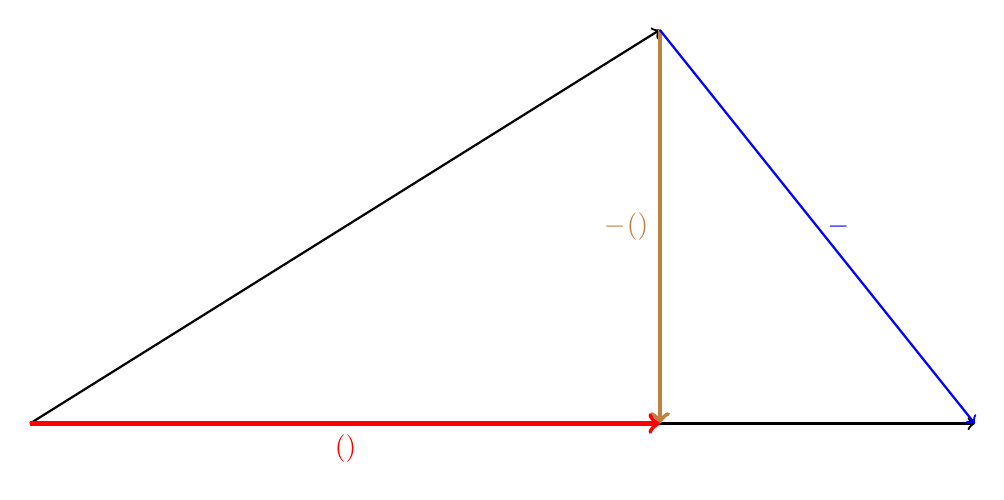
\begin{tikzpicture}
    \draw[->, thick]{(0, 0) -- node[below] {\( \vw \)} (12, 0)};
    \draw[->, thick]{(0, 0) -- node[above] {\( \vv \)} (8, 5)};
    \draw[->, brown, ultra thick]{(8, 5) -- node[left] {\(\vv - \proj_{\vw}(\vv)\)} (8, 0)};
    \draw[->, red, ultra thick]{(0, 0) -- node[below] {\( \proj_{\vw}(\vv) \)} (8, 0)};
    \draw[->, blue, thick]{(8, 5) -- node[right]{\( \vv - \vw \)}(12, 0)};
\end{tikzpicture}
\end{center}

%
%
%
\subsection{Adjoints}

\paragraph{Covectors and Dual Space}
Fix some vector \( \vx \) in a product space \( VA. \)
Then, we know that the map \( \vc \mapsto \innerprod{v}{x} \) is a linear map
from \( V \) to \( \mathbb{F} \).
Maps of the form \( V \to \mathbb{F} \) are called covectorsl
The dual space is the set of all covectors, \( V^* \) and is isomorphic to \( V \).

Then, covector can be written as an inner product with some fixed vector.
In the real case, we have a canonical isomorphism between \( V \) and \( V^* \)

\paragraph{Raising and Lowering the Index}

Let \( (V, \innerprod{}{}) \) be a finite dimensional vector space
with a linear mapping \( T: V \to \mathbb{F} \).
Then, there exists some unique \( \vt \in V \) such that for all \( \vv \in V \),
\[
    T(\vv) = \innerprod{\vt}{\vv}.
\]

The isomorphism \( T \mapsto \vt \) is called raising the index, denoted
with \( \vt = T^\sharp \).
The inverse \( \vt \mapsto T \), with \( T(\vv) = \innerprod{\vt}{\vv} \)
is called lowering the index, denoted with \( T = \vt^\flat \).

For \( \mathbb{R}^n \) with the standard dot product, \( \vv^\flat = \vv^T \).
The dual-space then can just be thought of as corresponding row-vectors.
The complex case is out of scope but, features conjugate linearity and has
isomorphisms to the conjugate dual space \( \overline{V^*} \).

\paragraph{Adjoint}
In essence, the adjoint is a linear map that reverses inner products.
For a linear map \( T: V \to W \) on finite dimensional inner product spaces,
there exists a unique linear map \( T^* \) (the adjoint) such that \[
    \innerprod{\vv}{T(\vv)} = \innerprod{T^*(\vv)}{\vv}.
\]

\paragraph{Standard Real and Complex Adjoint}
For a linear map \( T \) with matrix \( A \), the adjoint is the conjugate transpose.
In the real case, this is just the transpose.
That is \( T^*(w) = \overline{A^t} \vw \).
We denote this as \( A^* \).

%
%
%
\subsection{Special Cases of Adjoints}

\paragraph{Special Linear Maps}
The following cases are for a linear map \( T: V \to V \).
\begin{itemize}
    \item \textbf{Unitary}: \( T^* = T^{-1} \)
    \item \textbf{Isometry}: Preserves lengths. That is, \( ||T(\vv)|| = ||\vv|| \).
    \item \textbf{Hermetian/Self-Adjoint}: \( T^* = T \)
\end{itemize}

\paragraph{Properties of Unitary Maps}
\begin{itemize}
    \item A map is unitary if and only if \( T^* \) is also unitary.
    \item The set of all unitary transformations forms a group under composition.
\end{itemize}

\paragraph{Equivalencies on Special Maps}
The following are all equivalent for a linear map \( T: V \to V \) on
and inner product space \( V \):
\begin{enumerate}
    \item \( T \) is an isometry (preserves length).
    \item \( T \) is unitary.
    \item \( T^* \) is an isometry.
    \item \( T \) preserves inner products: \( \innerprod{T(\vv)}{T(\vw)} = \innerprod{\vv}{\vw} \).
    \item If \( \set{\ve_1, \dots \ve_n} \) is an orthonormal basis,
        so is \( T(\ve_1),\dots T(\ve_n) \).
\end{enumerate}

\paragraph{Polarisation Identities}
The polarisation identities are a set of identities that relate inner products
to norms. For the real and complex cases, we have
\begin{align*}
    \mathbb{R}:& \innerprod{\vx}{\vy} = \frac{1}{4}\left(
        \norm*{\vx + \vy}^2 - \norm*{\vx - \vy}^2
    \right) \\
    \mathbb{C}:& \innerprod{\vx}{\vy} = \frac{1}{4}\left[
        \norm*{\vx + \vy}^2 - \norm*{\vx - \vy}^2
        + i \left(\norm*{\vx + i\vy} + \norm*{\vx -i\vy} \right)
    \right]
\end{align*} 

\paragraph{Matrix Representation of Special Maps}
For matrices, the special cases hold as follows for the complex case:
\begin{itemize}
    \item Unitary: \( A^* = A^{-1} \),
    \item Hermetian: \( A^* = A \).
\end{itemize}
For the real case,
\begin{itemize}
    \item Orthogonal: \( A^T = A^{-1} \),
    \item Symmetric: \( A^T = A \).
\end{itemize}
Thus, the columns of a \( p\times p \) matrix form an orthonormal basis
for \( \mathbb{C}^p \) if and only if \( A \) is unitary.
For the real case, orthogonality is enough.
This also holds for rows due to the transposition.

\subsection{QR Factorisations}

\paragraph{QR form}
For a \( p\times q \) matrix \( A \) of rank \( q \), we can write \[
    A = QR
\]
for some \( p\times q \) matrix \( Q \) with orthonormal columns and
and invertible upper-triangular matrix \( R \).